\chapter{Entropy Coding}
Entropy coding is a lossless data compression scheme based on symbols probability. This concept was first described by Claude E. Shannon in 1948 in his paper \textit{A~Mathematical Theory of Communication} \parencite{Shannon1948}.

Giving an extensive theoretical explanation of Entropy coding would require an entire thesis. Therefore, in this chapter we will define the most basic equations in Information Theory and we will also describe some well-known coding algorithms that will be relevant later. The interested reader should see reference \parencite{cover}.

\begin{figure}[h!]
\begin{center}
	\begin{tabular}{ @{} c @{} }
		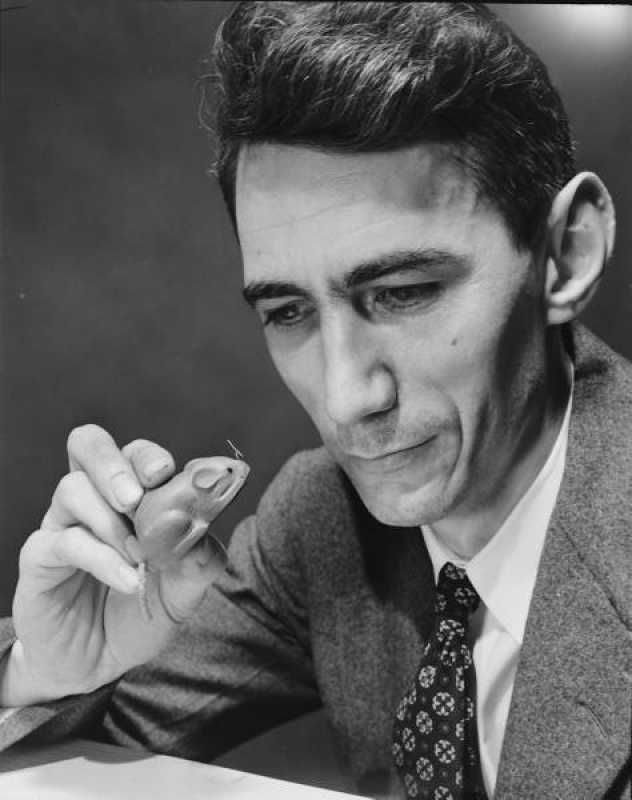
\includegraphics[scale=0.25]{images/Claude_Shannon_1776.jpg}\\
		\imagesource{DobriZheglov, CC BY-SA 4.0, via Wikimedia Commons.}
	\end{tabular}
\end{center}
\vspace*{-0.7em}
\caption{Picture of Claude E. Shannon staring at a mouse.}
\label{fig:shannon}
\end{figure}

\section{Information theory basics}
\subsection{Shannon entropy}
Given a discrete random variable $X$ with probability function $p(x)$, its Shannon entropy is defined as:

\begin{equation}
H(X) = - \sum_{i=1}^{n} p(x_i) \cdot \log_2 p(x_i) 
\end{equation}

This result represents the average level of information (or uncertainty) of the random variable $X$. It is expressed in \textit{bits}. Sometimes entropy is defined using the natural logarithm. In those situations the result is in \textit{nats}.


\subsubsection{Shannon's source coding theorem}
Shannon's source coding theorem establishes the theoretical limits to data compression, and a different meaning to Shannon entropy defined above. Formally, it states:

\begin{theorem}
Let $L_n^*$ be the expected codeword length per symbol of an optimal n-th order lossless data compression code (in bits/symbol). Let $(X_1, X_2, \dots, X_n )$ be a sequence of symbols from a stochastic process $X$. Then,

\begin{equation}
	\frac{H(X_1, X_2, \dots, X_n )}{n} \leq L_n^* < \frac{H(X_1, X_2, \dots, X_n )}{n} + \frac{1}{n}
\end{equation}

If $X$ is a stationary stochastic process,
\begin{equation}
	\lim_{n \to \infty} L_n^* = H(X)
\end{equation}
\end{theorem}

This theorem reveals a new interpretation of Shannon entropy: it is the average number of bits per symbol required to encode it.

\subsection{Differential entropy}
Given a continuous random variable X with a density $f(x)$ supported in $S$, its differential entropy is defined as:
\begin{equation} \label{eq:differential_entropy}
h(x) = - \int_{S}^{} f(x) \ln f(x) dx
\end{equation}

Notice that we have defined differential entropy using the natural logarithm, hence the result shall be expressed in \textit{nats}.

In some cases computing an explicit probability density function is too hard or even impossible. In these cases, an equivalent definition in terms of the quantile function $Q(p)$ can be used (see appendix \ref{entropy_proof}):
\begin{equation} \label{eq:differential_entropy_q}
h(p) = \int_{0}^{1} \ln Q'(p) dp
\end{equation}

This equation is specially useful in some entropy estimation techniques \parencite{Vasicek}.

\subsubsection{Maximum entropy}
Among all the real-valued distributions supported on $(-\infty, +\infty)$ with a specified variance $\sigma^2$, the normal distribution $N(\mu, \sigma^2)$ has maximum entropy:
\begin{equation}
h(x) = \frac{1}{2} \ln (2\sigma^2\pi) + \frac{1}{2}
\end{equation}

\section{Coding techniques}
There exist several techniques to assign bits to symbols. In general, one would be interested in a coding scheme which gives codewords with a mean length as close as possible to the Shannon limit. However, achieving the optimality might be too demanding in some scenarios, so other faster but suboptimal techniques have been developed.

In this section we will describe Golomb coding, a known technique used by several standards such as \acrshort{flac} or \acrshort{ccsds} 121.0. Besides, the \acrshort{fapec} entropy coder is highly inspired in Rice codes, a subset of the Golomb codes.

Before continuing, it is important to observe that there exist other entropy coding techniques which are more common than Golomb, for instance Huffman coding \parencite{cover}, arithmetic coding \parencite{MacKay} or more recently the Asymmetric Numeral System \parencite{ans}.

\subsection{Golomb coding} \label{golomb-coding}
\begin{comment}
Els codis de Rice (subconjunt dels codis de Golomb) van donar origen a FAPEC, així que és important comentar-los.
També són codis de prefix com el Huffman però poden no ser òptims \parencite{Golomb1966}.
\end{comment}

Golomb codes were first proposed by Solomon W. Golomb in 1966 in his article \textit{Run-Length Encodings} \parencite{Golomb1966}.

